\section{Measurement of inductance}
The measurement of inductance values will be done as separate part with all found resistors with
less than \(2100~\Omega\).
The methode of measurement is based on the growing of current by formula \(Il~=~Imax~\cdot~(1~-~\exp{\frac{-t}{\tau}})\) 
after switching on the current.
The time constant \(\tau = \frac{L}{R}\) is proportional to the inductance~\(L\), but reverse proportional to the
resistor~\(R\). 
The current can only measured indirectly with the potential drop of a resistor.
Unfortunately the time constant will be reduced additionally by the relative high resistance \(680~\Omega\),
for that the measurement of little inductance values is additionally made difficult with the 8 MHz clock.
To get the time constant, the voltage at the \(680~\Omega\) resistor will be monitored by the analog
comparator.
If the voltage drop at the \(680~\Omega\) resistor is higher than the voltage of the internal reference, this
event will be notified to the 16-bit counter, which is started at the same time of switching current on.
The counter will save the state of this event.
If the counter will overrun, this will be counted by the program.
After the event, the counter will be stopped by the program and the total time will be build with the saved
counter stage and the overflow counter.
The positive side of the coil will be switched from VCC to GND and hold in this stage until  monitoring 
of the voltages of both pins shows, that no current is detected.
The figure~\ref{fig:Inductance} shown a simplified diagram of the measurement situation.

\begin{figure}[H]
\centering

\includegraphics[]{../FIG/Inductance.eps}
\caption{Measurement of inductances with the comparator}
\label{fig:Inductance}
\end{figure}

With the supply voltage VCC and the sum of all resistors in the electric circuit the maximum current Imax and from
that the percentage of the reference voltage to the maximum voltage at the \(680~\Omega\) resistor can be calculated
\(Umax~=~Imax~\cdot~(680~+~19)\) .
With the formula \(L~=~-\frac{t~\cdot~Rges}{\log{(1~-~\frac{Uref}{Umax})}}\) the inductance can be calculated.
The natural logarithm will be taken out of a build in table.
In order to also measure lower inductance values, the \(680 \Omega\) resistor will be omitted in the current loop,
if the resistance value of the inductor is measured with less than \(24 \Omega\).
Only the output resistance of the port (\(19 \Omega\)) will be used for measurement of the current.
In this special case the peak current will be greater than the value, that the specification of the ATmega allows.
Because this will be true only for a very short time, I expect no damage of the ATmega ports.
To avoid a longer time with excessive current, the additional measurement with delayed start of the counter will always be
done with the \(680 \Omega\) resistor.
To get better fitting measurement results, a zero offset of 6 is subtract from the counter reading, 
if the measurement is done without the \(680 \Omega\) resistor. Otherwise a zero offset of 8 is subtracted.


With great inductance values the parasitic capacity can cause a quick rise of current, so that the comparator
will responce inmmediately.
To get the value of the inductance anyway, the measurement will be repeated with a delayed start of the counter.
With this methode the voltage grow caused by the current increase of the inductor will be detected by the
analog comparator instead of the current peak of the parasitic capacity.
The measurements are always done in both current directions.
The program will select the higher result of measurement in the same current direction, but the
lower result of the different current direction as the displayed result.

\subsection{Results of the inductance measurements}
The figure~\ref{fig:Induct328p} shows the results of the measurement of different inductors.
The Inductors above \(1 H\) are relays or primary sides of power transformers, for which
measurements are difficult because the iron core has residual remanence.


\begin{figure}[H]
\centering
% GNUPLOT: LaTeX picture with Postscript
\begingroup
  \makeatletter
  \providecommand\color[2][]{%
    \GenericError{(gnuplot) \space\space\space\@spaces}{%
      Package color not loaded in conjunction with
      terminal option `colourtext'%
    }{See the gnuplot documentation for explanation.%
    }{Either use 'blacktext' in gnuplot or load the package
      color.sty in LaTeX.}%
    \renewcommand\color[2][]{}%
  }%
  \providecommand\includegraphics[2][]{%
    \GenericError{(gnuplot) \space\space\space\@spaces}{%
      Package graphicx or graphics not loaded%
    }{See the gnuplot documentation for explanation.%
    }{The gnuplot epslatex terminal needs graphicx.sty or graphics.sty.}%
    \renewcommand\includegraphics[2][]{}%
  }%
  \providecommand\rotatebox[2]{#2}%
  \@ifundefined{ifGPcolor}{%
    \newif\ifGPcolor
    \GPcolortrue
  }{}%
  \@ifundefined{ifGPblacktext}{%
    \newif\ifGPblacktext
    \GPblacktexttrue
  }{}%
  % define a \g@addto@macro without @ in the name:
  \let\gplgaddtomacro\g@addto@macro
  % define empty templates for all commands taking text:
  \gdef\gplbacktext{}%
  \gdef\gplfronttext{}%
  \makeatother
  \ifGPblacktext
    % no textcolor at all
    \def\colorrgb#1{}%
    \def\colorgray#1{}%
  \else
    % gray or color?
    \ifGPcolor
      \def\colorrgb#1{\color[rgb]{#1}}%
      \def\colorgray#1{\color[gray]{#1}}%
      \expandafter\def\csname LTw\endcsname{\color{white}}%
      \expandafter\def\csname LTb\endcsname{\color{black}}%
      \expandafter\def\csname LTa\endcsname{\color{black}}%
      \expandafter\def\csname LT0\endcsname{\color[rgb]{1,0,0}}%
      \expandafter\def\csname LT1\endcsname{\color[rgb]{0,1,0}}%
      \expandafter\def\csname LT2\endcsname{\color[rgb]{0,0,1}}%
      \expandafter\def\csname LT3\endcsname{\color[rgb]{1,0,1}}%
      \expandafter\def\csname LT4\endcsname{\color[rgb]{0,1,1}}%
      \expandafter\def\csname LT5\endcsname{\color[rgb]{1,1,0}}%
      \expandafter\def\csname LT6\endcsname{\color[rgb]{0,0,0}}%
      \expandafter\def\csname LT7\endcsname{\color[rgb]{1,0.3,0}}%
      \expandafter\def\csname LT8\endcsname{\color[rgb]{0.5,0.5,0.5}}%
    \else
      % gray
      \def\colorrgb#1{\color{black}}%
      \def\colorgray#1{\color[gray]{#1}}%
      \expandafter\def\csname LTw\endcsname{\color{white}}%
      \expandafter\def\csname LTb\endcsname{\color{black}}%
      \expandafter\def\csname LTa\endcsname{\color{black}}%
      \expandafter\def\csname LT0\endcsname{\color{black}}%
      \expandafter\def\csname LT1\endcsname{\color{black}}%
      \expandafter\def\csname LT2\endcsname{\color{black}}%
      \expandafter\def\csname LT3\endcsname{\color{black}}%
      \expandafter\def\csname LT4\endcsname{\color{black}}%
      \expandafter\def\csname LT5\endcsname{\color{black}}%
      \expandafter\def\csname LT6\endcsname{\color{black}}%
      \expandafter\def\csname LT7\endcsname{\color{black}}%
      \expandafter\def\csname LT8\endcsname{\color{black}}%
    \fi
  \fi
  \setlength{\unitlength}{0.0500bp}%
  \begin{picture}(7200.00,5040.00)%
    \gplgaddtomacro\gplbacktext{%
      \csname LTb\endcsname%
      \put(814,704){\makebox(0,0)[r]{\strut{}-20}}%
      \csname LTb\endcsname%
      \put(814,1213){\makebox(0,0)[r]{\strut{}-15}}%
      \csname LTb\endcsname%
      \put(814,1722){\makebox(0,0)[r]{\strut{}-10}}%
      \csname LTb\endcsname%
      \put(814,2231){\makebox(0,0)[r]{\strut{}-5}}%
      \csname LTb\endcsname%
      \put(814,2740){\makebox(0,0)[r]{\strut{} 0}}%
      \csname LTb\endcsname%
      \put(814,3248){\makebox(0,0)[r]{\strut{} 5}}%
      \csname LTb\endcsname%
      \put(814,3757){\makebox(0,0)[r]{\strut{} 10}}%
      \csname LTb\endcsname%
      \put(814,4266){\makebox(0,0)[r]{\strut{} 15}}%
      \csname LTb\endcsname%
      \put(814,4775){\makebox(0,0)[r]{\strut{} 20}}%
      \csname LTb\endcsname%
      \put(946,484){\makebox(0,0){\strut{}10u}}%
      \csname LTb\endcsname%
      \put(1783,484){\makebox(0,0){\strut{}100u}}%
      \csname LTb\endcsname%
      \put(2619,484){\makebox(0,0){\strut{}1m}}%
      \csname LTb\endcsname%
      \put(3456,484){\makebox(0,0){\strut{}10m}}%
      \csname LTb\endcsname%
      \put(4293,484){\makebox(0,0){\strut{}100m}}%
      \csname LTb\endcsname%
      \put(5130,484){\makebox(0,0){\strut{}1 }}%
      \csname LTb\endcsname%
      \put(5966,484){\makebox(0,0){\strut{}10 }}%
      \csname LTb\endcsname%
      \put(6803,484){\makebox(0,0){\strut{}100 }}%
      \put(176,2739){\rotatebox{-270}{\makebox(0,0){\strut{}Error / Percent}}}%
      \put(3874,154){\makebox(0,0){\strut{}Inductance value / H}}%
      \put(3874,4665){\makebox(0,0){\strut{}}}%
    }%
    \gplgaddtomacro\gplfronttext{%
      \csname LTb\endcsname%
      \put(5690,4594){\makebox(0,0)[r]{\strut{}328p}}%
      \csname LTb\endcsname%
      \put(5690,4358){\makebox(0,0)[r]{\strut{}328}}%
      \csname LTb\endcsname%
      \put(5690,4122){\makebox(0,0)[r]{\strut{}168p}}%
      \csname LTb\endcsname%
      \put(5690,3886){\makebox(0,0)[r]{\strut{}168a}}%
      \csname LTb\endcsname%
      \put(5690,3650){\makebox(0,0)[r]{\strut{}168}}%
    }%
    \gplbacktext
    \put(0,0){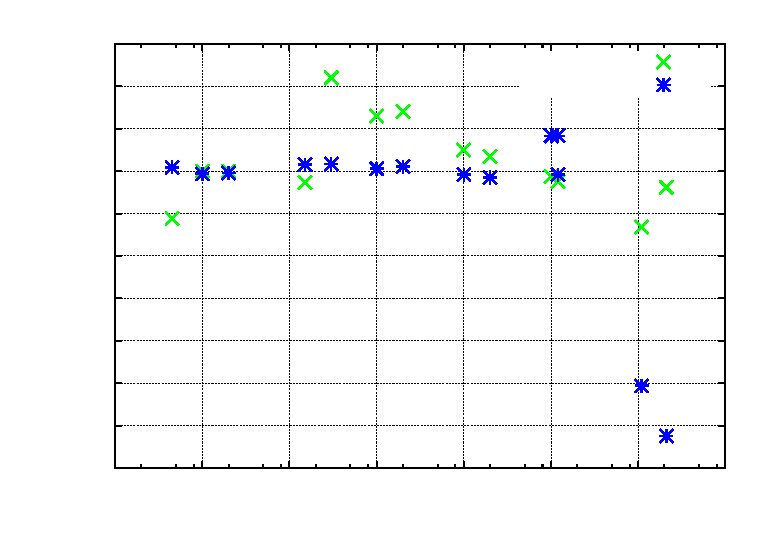
\includegraphics{../GNU/induct328p}}%
    \gplfronttext
  \end{picture}%
\endgroup

\caption{Error of inductance measurement of 15 different ATmega}
\label{fig:Induct328p}
\end{figure}

